The first computational models created by computer scientists come from Automata Theory, which is the study of abstract automata or `machines' (\cite{HopcroftJohnE.2014Itat}). In the 1930s Alan Turing and Alonzo Church studied a particular type of automata known as \textbf{finite-state automata} and built on this with the development of the \textbf{Turing Machine}. We utilise this model due to its flexibility and versatility. There are many variations on the model, but we begin with the one-tape \textbf{Deterministic Turing Machine} (DTM).

The DTM contains a \textbf{finite state control}, a \textbf{read-write head}, and an infinite sequence of \textbf{tape squares}, labelled \(\dots,-2,-1,0,1,2,\dots\). By convention we always set the start of our input at position 1, which we refer to as the \textbf{initialisation} of our Turing Machine.

\begin{figure}[h]
\centering

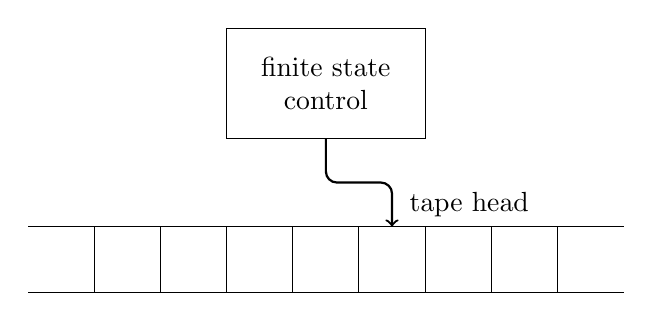
\begin{tikzpicture}[scale=1.4]
    \draw (5.5,1) rectangle (7.3,2);
    
    \node[text width = 2cm, align = center] at (6.4,1.5) {finite state control};

    \draw[thick] [->] {[rounded corners] (6.4,1) -- (6.4,0.6) -- (7,0.6) -- (7,0.2)};

    \node at (7.7,0.4) {tape head};

	\draw (3.7,0.2) -- (4.3,0.2) -- (4.3,-0.4) -- (3.7,-0.4);
	\draw (4.3,0.2) rectangle (4.9,-0.4);
	\draw (4.9,0.2) rectangle (5.5,-0.4);
	\draw (5.5,0.2) rectangle (6.1,-0.4);
	\draw (6.1,0.2) rectangle (6.7,-0.4);
	\draw (6.7,0.2) rectangle (7.3,-0.4);
	\draw (7.3,0.2) rectangle (7.9,-0.4);
	\draw (7.9,0.2) rectangle (8.5,-0.4);
	\draw (9.1,-0.4) -- (8.5,-0.4) -- (8.5,0.2) -- (9.1,0.2);

\end{tikzpicture}


\begin{tikzpicture}[scale=1.4]
	
	\node at (4.6,0.9) {-3};
	\node at (5.2,0.9) {-2};
	\node at (5.8,0.9) {-1};
	\node at (6.4,0.9) {0};
	\node at (7.0,0.9) {1};
	\node at (7.6,0.9) {2};
	\node at (8.2,0.9) {3};

\end{tikzpicture}

\caption{A one-tape DTM that has been initialised.}
\label{fig:DTMModel}
\end{figure}

There is also a set number of states that the DTM can be in, which influence the action the finite state control takes. When the tape head reads a cell, based on the value of the cell and the state it will do three things:

\begin{itemize}
    \item Rewrite the item on the tape head;
    \item Choose to move the tape forwards or backwards one cell, or stay on the same cell;
    \item Optionally change the state of the DTM.
\end{itemize}

\noindent We now provide a formal definition.

\begin{definition}
    (\cite{GareyMichaelR1979Cai:}) A \textbf{program} in a one-tape Deterministic Turing Machine (DTM) is a tuple \((\Gamma,Q,\delta)\) such that:
    \begin{itemize}
        \item \(\Gamma\) is a finite set of tape symbols, including a subset $\Sigma \subset \Gamma$ \textbf{input symbols} and a \textbf{blank symbol} $b \in \Gamma \setminus \Sigma$;
        \item \(Q\) is a finite set of states, including a unique start-state \(q_0\) and two unique halt-states \(q_Y\) and \(q_N\);
        \item \(\delta\) represents a transition function \(\delta:Q \setminus \{q_Y,q_N\}
        \times \Gamma \rightarrow Q \times \Gamma \times \{-1,0 +1\}\).
    \end{itemize}
    In our set of tape symbols, the subset $\Sigma$ is referred to as an \textbf{alphabet}.
\end{definition}

For the sake of brevity, in this report we refer to a program in a one-tape DTM as a DTM. Now that we have defined a program, what is left is to consider the possible set of inputs into a program:

\begin{definition}
    Consider an alphabet \(\Sigma = \{\sigma_1,\sigma_2,\dots,\sigma_n\}\). We denote \(\Sigma^*\) to be the set of all finite strings of symbols from \(\Sigma\). A \textbf{language} is a subset \(L \subseteq \Sigma^*\) and an \textbf{instance} or \textbf{input} is an element $x \in \Sigma^*$.
\end{definition}

\begin{remark}
    By convention the string of length $0$ is given by $\epsilon$.
\end{remark}
As an example, for the binary alphabet \(\{0,1\}\) we have \[\{0,1\}^* = \{\epsilon, 0, 1, 00, 01, 10, 11, 000, 001, 010, 011, 100, \dots\}.\]

\subsubsection{Encodings}\label{sec:Encodings}
The physical manifestation of a Turing Machine tends to take the form of either an electronic computer or a physical tape passing through a tape head. In either case, the tape head can only read up to two pieces of information. In the case of an electronic TM, either there is electricity passing through the tape head or no electricity. In the case of a paper tape, there is either a punched hole or no punched hole. Therefore, for our Turing Machine model to be faithful to a real-world model, we implement it using the alphabet $\{0,1\}$.

There are many different items that we will want to represent in our DTM, which we need to represent through this alphabet; we use a process called \textbf{encoding} to represent them.

To represent a number, we note that we can use a representation known as \textbf{binary}. Typically we use a system called \textbf{base 10}, which means that a number like $354$ can be also written as $3 \cdot 10^2+5 \cdot 10^1 + 4 \cdot 10^0$. We can represent a number in base 2, or \textbf{binary}, in a similar way:
\begin{align*}
    9 \text{  in base } 10 &= 1 \cdot 2^3 + 0 \cdot 2^2 + 0 \cdot 2^1 + 1 \cdot 2^0\\
    &=1001 \text{ in base } 2.
\end{align*}

We can also represent graphs in binary; for an undirected graph, we can label the vertices with some indexing set and create a matrix such that
\begin{align*}
    a_{i,j} =
    \begin{cases}
        1 \text{ if there is an edge between $v_i$ and $v_j$}\\
        0 \text{ otherwise}
    \end{cases}
\end{align*}

Such a matrix is called an \textbf{adjacency matrix}. We then input it row by row into the TM, which acts as an encoding for our graph, as shown in Figure \ref{fig:AdjacencyMatrix}.

\begin{figure}
    \centering
    \parbox{2in}{
    \begin{equation*}
    \begin{pmatrix}
        0 & 1 & 0 & 1 \\
        1 & 0 & 1 & 1 \\
        0 & 1 & 0 & 0 \\
        1 & 1 & 0 & 0 \\
    \end{pmatrix}
    \end{equation*}}
    \begin{minipage}{2in}
    \begin{tikzpicture}[baseline(10.base), thick, main/.style = {draw,circle}]

    \node (1) [circle,draw] at (0,2) {$v_1$};
    \node (2) [circle,draw] at (2,2) {$v_2$};
    \node (3) [circle,draw] at (2,0) {$v_3$};
    \node (4) [circle,draw] at (0,0) {$v_4$};

    \graph{(1) -- (2) -- (4) -- (1)};
    \graph{(2) -- (3)};
    \end{tikzpicture}
    \end{minipage}

    
    \caption{An adjacency matrix and its corresponding graph.}
    \label{fig:AdjacencyMatrix}
\end{figure}

\subsubsection{Decision problems}
One use case of the Turing Machine is to solve problems.

\begin{definition}
    A decision problem, $\Pi$, consists of a set $D_{\Pi}$ of \textbf{instances} and a subset $Y_\Pi \subseteq D_\Pi$ of \textbf{yes-instances.}
\end{definition}

A common way to give decision problems (and how they will be referred to in this report) is in the \textbf{instance-problem} form. Here is an example decision problem:

\decisionproblem{Divisibility by four}{A natural number $x$.}{Is $x$ divisible by $4$?}

\begin{remark}\label{remark:DecisionProblem-Language}
    Any decision problem describes a language, as the set of yes-instances (given by instances for which the answer to the problem is `yes') is a subset of all possible instances in $\Pi$.
\end{remark}

\begin{definition} \label{def:Computation}
    Let $\Sigma$ be the alphabet for a program $M$ in a Deterministic Turing Machine, and consider an instance \(x \in \Sigma^*\). We say that $M$ \textbf{halts, computes $x$} or \textbf{decides $x$} if there exists $T \in \mathbb{N}$ such that for all $t\geq T$, the state, location and contents of all cells of $M$ after $t$ steps is equal to that after $t+1$ steps. Furthermore, we say that
    \begin{itemize}
        \item $M$ \textbf{accepts} $x$ if $M$ halts on state $q_Y$;
        \item $M$ \textbf{rejects} $x$ if $M$ halts on state $q_N$;
        \item The language $L_M$ \textbf{recognised} by $M$ is given by the set \[L_M = \{x \in \Sigma^*: M \text{ accepts } x\}\]
    \end{itemize}
    
\end{definition}

\begin{example}
    We can compute the decision problem \textsc{Divisibility by four} using a Turing Machine.
    
    Set \(\Sigma = \{0,1\}\) and let \(Q = \{q_0,q_1,q_2,q_Y,q_N\}\). Lastly, set our transition function as below:

    \begin{table}[h]
    \centering
        \begin{tabular}{|c|c|c|c|}
            \hline
            & \(0\) & \(1\) & \(b\) \\
            \hline
            \(q_0\) & \((q_0,0,+1)\) & \((q_0,b,+1)\) & \((q_1,1,-1)\) \\
            \hline
            \(q_1\) & \((q_2,0,-1)\) & \((q_N, 1, +1)\) & \((q_N,b,+1)\) \\
            \hline
            \(q_2\) & \((q_Y,0,+1)\) & \((q_N,1,+1)\) & \((q_N,b,+1)\)\\
            \hline
        \end{tabular}\\
        \caption{A table of the transition function for $M$. An output from the transition function is taken by taking the input symbol along the top row and the current state along the left hand column and reading the corresponding cell.}
        \label{table:DivisibilityByFourTransitionTable}
    \end{table}
    Consider the number $28$. We know that $28$ is equal to $7$ times $4$, so it should return a successful result. Indeed, it does:

    \begin{center}

\begin{tikzpicture}[scale=1.4]
    \node at (3.4,1.5) {Current state};
    \node at (6.4,1.5) {Tape};
    \node at (10,1.5) {Transition function}

	\draw (3.7,1.2) -- (4.3,1.2) -- (4.3,0.6) -- (3.7,0.6);
	\draw (4.3,1.2) rectangle (4.9,0.6);
	\draw[fill=lightgray, thick] (4.9,1.2) rectangle (5.5,0.6);
	\draw (5.5,1.2) rectangle (6.1,0.6);
	\draw (6.1,1.2) rectangle (6.7,0.6);
	\draw (6.7,1.2) rectangle (7.3,0.6);
	\draw (7.3,1.2) rectangle (7.9,0.6);
	\draw (7.9,1.2) rectangle (8.5,0.6);
	\draw (9.1,0.6) -- (8.5,0.6) -- (8.5,1.2) -- (9.1,1.2);
	
	\node at (3.4,0.9) {\(q_0\)};
	\node at (4.6,0.9) {\(b\)};
	\node at (5.2,0.9) {$1$};
	\node at (5.8,0.9) {$1$};
	\node at (6.4,0.9) {$1$};
	\node at (7.0,0.9) {$0$};
	\node at (7.6,0.9) {$0$};
	\node at (8.2,0.9) {\(b\)};
	\node at (10,0.9) {\((q_0,1,+1)\)};
% ROW 2
	\draw (3.7,0.5) -- (4.3,0.5) -- (4.3,-0.1) -- (3.7,-0.1);
	\draw (4.3,0.5) rectangle (4.9,-0.1);
	\draw (4.9,0.5) rectangle (5.5,-0.1);
	\draw[fill=lightgray, thick] (5.5,0.5) rectangle (6.1,-0.1);
	\draw (6.1,0.5) rectangle (6.7,-0.1);
	\draw (6.7,0.5) rectangle (7.3,-0.1);
	\draw (7.3,0.5) rectangle (7.9,-0.1);
	\draw (7.9,0.5) rectangle (8.5,-0.1);
	\draw (9.1,-0.1) -- (8.5,-0.1) -- (8.5,0.5) -- (9.1,0.5);
	
	\node at (3.4,0.2) {\(q_0\)};
	\node at (4.6,0.2) {\(b\)};
	\node at (5.2,0.2) {$1$};
	\node at (5.8,0.2) {$1$};
	\node at (6.4,0.2) {$1$};
	\node at (7.0,0.2) {$0$};
	\node at (7.6,0.2) {$0$};
	\node at (8.2,0.2) {\(b\)};
	\node at (10,0.2) {\((q_0,1,+1)\)};
% ROW 3
	\draw (3.7,-0.2) -- (4.3,-0.2) -- (4.3,-0.8) -- (3.7,-0.8);
	\draw (4.3,-0.2) rectangle (4.9,-0.8);
	\draw (4.9,-0.2) rectangle (5.5,-0.8);
	\draw (5.5,-0.2) rectangle (6.1,-0.8);
	\draw[fill=lightgray, thick] (6.1,-0.2) rectangle (6.7,-0.8);
	\draw (6.7,-0.2) rectangle (7.3,-0.8);
	\draw (7.3,-0.2) rectangle (7.9,-0.8);
	\draw (7.9,-0.2) rectangle (8.5,-0.8);
	\draw (9.1,-0.8) -- (8.5,-0.8) -- (8.5,-0.2) -- (9.1,-0.2);
	
	\node at (3.4,-0.5) {\(q_0\)};
	\node at (4.6,-0.5) {\(b\)};
	\node at (5.2,-0.5) {$1$};
	\node at (5.8,-0.5) {$1$};
	\node at (6.4,-0.5) {$1$};
	\node at (7.0,-0.5) {$0$};
	\node at (7.6,-0.5) {$0$};
	\node at (8.2,-0.5) {\(b\)};
	\node at (10,-0.5) {\((q_0,1,+1)\)};

% ROW 4

    \draw (3.7,-0.9) -- (4.3,-0.9) -- (4.3,-1.5) -- (3.7,-1.5);
    \draw (4.3,-0.9) rectangle (4.9,-1.5);
    \draw (4.9,-0.9) rectangle (5.5,-1.5);
    \draw (5.5,-0.9) rectangle (6.1,-1.5);
    \draw (6.1,-0.9) rectangle (6.7,-1.5);
    \draw[fill=lightgray, thick] (6.7,-0.9) rectangle (7.3,-1.5);
    \draw (7.3,-0.9) rectangle (7.9,-1.5);
    \draw (7.9,-0.9) rectangle (8.5,-1.5);
    \draw (9.1,-1.5) -- (8.5,-1.5) -- (8.5,-0.9) -- (9.1,-0.9);

    \node at (3.4,-1.2) {\(q_0\)};
    \node at (4.6,-1.2) {\(b\)};
    \node at (5.2,-1.2) {$1$};
    \node at (5.8,-1.2) {$1$};
    \node at (6.4,-1.2) {$1$};
    \node at (7.0,-1.2) {$0$};
    \node at (7.6,-1.2) {$0$};
    \node at (8.2,-1.2) {\(b\)};
    \node at (10,-1.2) {\((q_0,0,+1)\)};

% ROW 5

	\draw (3.7,-1.6) -- (4.3,-1.6) -- (4.3,-2.2) -- (3.7,-2.2);
	\draw (4.3,-1.6) rectangle (4.9,-2.2);
	\draw (4.9,-1.6) rectangle (5.5,-2.2);
	\draw (5.5,-1.6) rectangle (6.1,-2.2);
	\draw (6.1,-1.6) rectangle (6.7,-2.2);
	\draw (6.7,-1.6) rectangle (7.3,-2.2);
	\draw[fill=lightgray, thick] (7.3,-1.6) rectangle (7.9,-2.2);
	\draw (7.9,-1.6) rectangle (8.5,-2.2);
	\draw (9.1,-2.2) -- (8.5,-2.2) -- (8.5,-1.6) -- (9.1,-1.6);
	
	\node at (3.4,-1.9) {\(q_0\)};
	\node at (4.6,-1.9) {\(b\)};
	\node at (5.2,-1.9) {$1$};
	\node at (5.8,-1.9) {$1$};
	\node at (6.4,-1.9) {$1$};
	\node at (7.0,-1.9) {$0$};
	\node at (7.6,-1.9) {$0$};
	\node at (8.2,-1.9) {\(b\)};
	\node at (10,-1.9) {\((q_0,0,+1)\)};

% ROW 6

	\draw (3.7,-2.3) -- (4.3,-2.3) -- (4.3,-2.9) -- (3.7,-2.9);
	\draw (4.3,-2.3) rectangle (4.9,-2.9);
	\draw (4.9,-2.3) rectangle (5.5,-2.9);
	\draw (5.5,-2.3) rectangle (6.1,-2.9);
	\draw (6.1,-2.3) rectangle (6.7,-2.9);
	\draw (6.7,-2.3) rectangle (7.3,-2.9);
	\draw (7.3,-2.3) rectangle (7.9,-2.9);
	\draw[fill=lightgray, thick] (7.9,-2.3) rectangle (8.5,-2.9);
	\draw (9.1,-2.9) -- (8.5,-2.9) -- (8.5,-2.3) -- (9.1,-2.3);
	
	\node at (3.4,-2.6) {\(q_0\)};
	\node at (4.6,-2.6) {\(b\)};
	\node at (5.2,-2.6) {$1$};
	\node at (5.8,-2.6) {$1$};
	\node at (6.4,-2.6) {$1$};
	\node at (7.0,-2.6) {$0$};
	\node at (7.6,-2.6) {$0$};
	\node at (8.2,-2.6) {\(b\)};
	\node at (10,-2.6) {\((q_1,b,-1)\)};

% ROW 7

	\draw (3.7,-3.0) -- (4.3,-3.0) -- (4.3,-3.6) -- (3.7,-3.6);
	\draw (4.3,-3.0) rectangle (4.9,-3.6);
	\draw (4.9,-3.0) rectangle (5.5,-3.6);
	\draw (5.5,-3.0) rectangle (6.1,-3.6);
	\draw (6.1,-3.0) rectangle (6.7,-3.6);
	\draw (6.7,-3.0) rectangle (7.3,-3.6);
	\draw[fill=lightgray, thick] (7.3,-3.0) rectangle (7.9,-3.6);
	\draw (7.9,-3.0) rectangle (8.5,-3.6);
	\draw (9.1,-3.6) -- (8.5,-3.6) -- (8.5,-3.0) -- (9.1,-3.0);
	
	\node at (3.4,-3.3) {\(q_1\)};
	\node at (4.6,-3.3) {\(b\)};
	\node at (5.2,-3.3) {$1$};
	\node at (5.8,-3.3) {$1$};
	\node at (6.4,-3.3) {$1$};
	\node at (7.0,-3.3) {$0$};
	\node at (7.6,-3.3) {$0$};
	\node at (8.2,-3.3) {\(b\)};
	\node at (10,-3.3) {\((q_2,0,-1)\)};

% ROW 8

	\draw (3.7,-3.7) -- (4.3,-3.7) -- (4.3,-4.3) -- (3.7,-4.3);
	\draw (4.3,-3.7) rectangle (4.9,-4.3);
	\draw (4.9,-3.7) rectangle (5.5,-4.3);
	\draw (5.5,-3.7) rectangle (6.1,-4.3);
	\draw (6.1,-3.7) rectangle (6.7,-4.3);
	\draw[fill=lightgray, thick] (6.7,-3.7) rectangle (7.3,-4.3);
	\draw (7.3,-3.7) rectangle (7.9,-4.3);
	\draw (7.9,-3.7) rectangle (8.5,-4.3);
	\draw (9.1,-4.3) -- (8.5,-4.3) -- (8.5,-3.7) -- (9.1,-3.7);
	
	\node at (3.4,-4.0) {\(q_2\)};
	\node at (4.6,-4.0) {\(b\)};
	\node at (5.2,-4.0) {$1$};
	\node at (5.8,-4.0) {$1$};
	\node at (6.4,-4.0) {$1$};
	\node at (7.0,-4.0) {$0$};
	\node at (7.6,-4.0) {$0$};
	\node at (8.2,-4.0) {\(b\)};
	\node at (10,-4.0) {\((q_Y,0,+1)\)};
\end{tikzpicture}

\textbf{SUCCESS}

\end{center}

    By inspection of the transition function, it can be seen that the program recognises the language \[L_M = \{x \in \{0,1\}^*:\text{The two rightmost symbols of $x$ are both 0}\} \text{.}\]
\end{example}